\documentclass[crop,tikz]{standalone}
\usetikzlibrary{backgrounds}
\colorlet{blue}{cyan}
\tikzset{
  inverted/.style = {
    color=white,
    background rectangle/.style={fill},
    show background rectangle
  }
}

\usetikzlibrary{angles}
\usepackage{pgfplots}
\pgfplotsset{compat=1.18}

\pgfplotsset{
  inverted/.style = {
    every axis legend/.append style={
      draw=white,
      fill=black,
      text=white
    }
  },
}

\begin{document}
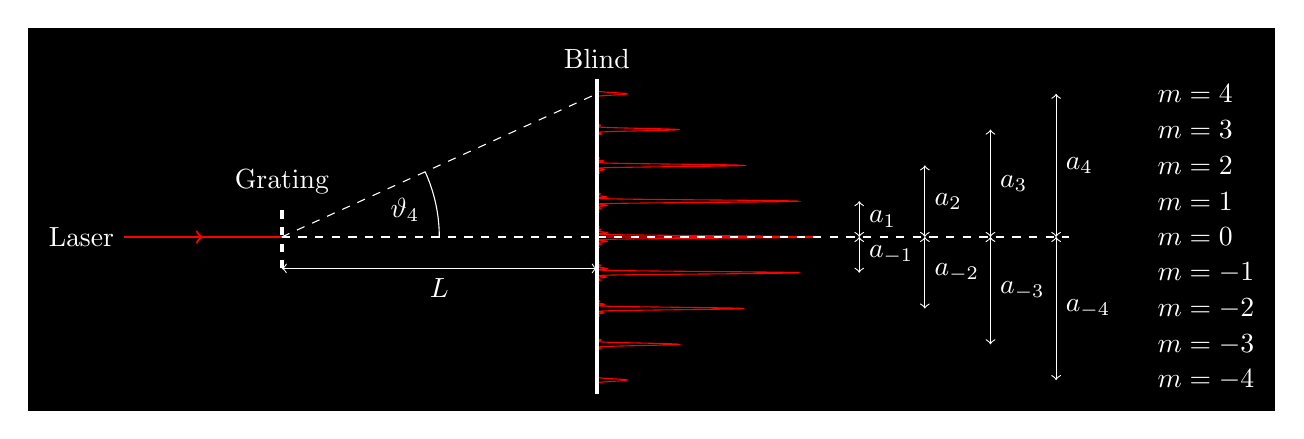
\begin{tikzpicture}[inverted,inverted]
  \pgfmathsetmacro{\nmax}{4};
  \pgfmathsetmacro{\nlines}{12};
  \pgfmathsetmacro{\xgrating}{0};
  \pgfmathsetmacro{\xblind}{4};
  \pgfmathsetmacro{\xscale}{1.1};
  \pgfmathsetmacro{\gratingheight}{0.8};
  \pgfmathsetmacro{\aone}{pi*4/(2*pi*\xscale*\nmax)}; % pi * width of plot / (xmax - xmin)
  % laser
  \draw[thick,red,->] (-2,0) node[left,white] {Laser} -- (-1,0);
  \draw[thick,red] (-1,0) -- (0,0);
  % grating
  \draw[ultra thick,dashed] (0,{-\gratingheight/2}) -- (0,{\gratingheight/2}) node[above] {Grating};
  % length
  \draw[<->] ({\xgrating},{-\gratingheight/2}) -- node[below] {$L$} ++({\xblind-\xgrating},0);
  % intensity distribution
  \begin{axis}[inverted,
    width=4cm,
    height=3cm,
    scale only axis,
    anchor=origin,
    rotate around={-90:(current axis.origin)},
    yshift=4cm,
    axis lines=none,
    domain={-\nmax*\xscale*pi}:{\nmax*\xscale*pi},
    xmin={-\nmax*\xscale*pi}, xmax={\nmax*\xscale*pi},
    ymin=0,
    samples=1001,
    ]
    \addplot[red,smooth] { sin(10*x)^2/((10*x)^2) * (sin(deg(\nlines*x))/sin(deg(x)))^2 };
  \end{axis}
  % blind
  \draw[ultra thick] (\xblind,-2) -- (\xblind,2) node[above] {Blind};
  % draw orders
  \foreach \m in {-\nmax,...,\nmax} {
    \node[right] at (11,{\m*\aone}) {$m=\m$};
  }
  \foreach \m in {1,...,\nmax} {
    \draw[<->] ({\xgrating + \xblind + 3 - 0.5 + \m/1.2},0) -- node[right] {$a_{\m}$}  ++ (0,{ \m*\aone});
    \draw[<->] ({\xgrating + \xblind + 3 - 0.5 + \m/1.2},0) -- node[right] {$a_{-\m}$} ++ (0,{-\m*\aone});
  }
  % draw axis and angle
  \coordinate (O) at ({\xblind},0);
  \coordinate (G) at (0,0);
  \coordinate (A) at ({\xblind},{\aone*\nmax});
  \draw[dashed] (G) -- (10,0);
  \draw[dashed] (G) -- (A);
  \pic[draw,pic text={$\vartheta_{\nmax}$},angle radius=2cm,angle eccentricity=0.8] {angle = O--G--A};
\end{tikzpicture}
\end{document}
